\chapter{Development and testing}
\label{chp:testing}
\noindent
The development of this thesis has been conducted in close collaboration with cardiac surgeons surgeons who are the main stakeholders of the project.

\section{Feedbacks from surgeons}
\noindent
The development of this thesis has been conducted in close collaboration with cardiac surgeons surgeons who are the main stakeholders of the project.
The development followed an iterative approach, Through a series of iterative meetings and discussions with the surgeons, we could assure the alignment of the software being developed with the requirements.\\
During the year of development, periodic testing sessions have been organized to assess the current state of the project and decide some development details, mainly concerning the user experience. Some of these sessions involved a reduced number of users, while others were done inviting a group of people to recreate the setting of a real lesson.
These collaborative sessions provided an opportunity to gather detailed feedback, which was then systematically integrated into the design and implementation phases.
This ongoing dialogue not only allowed for continuous improvement but also fostered a multidisciplinary approach.\\
The iterative development process led to a solution that is both technologically robust and highly tailored to the specific needs and expectations of the end users.\\


\begin{figure}[ht]
  \centering
  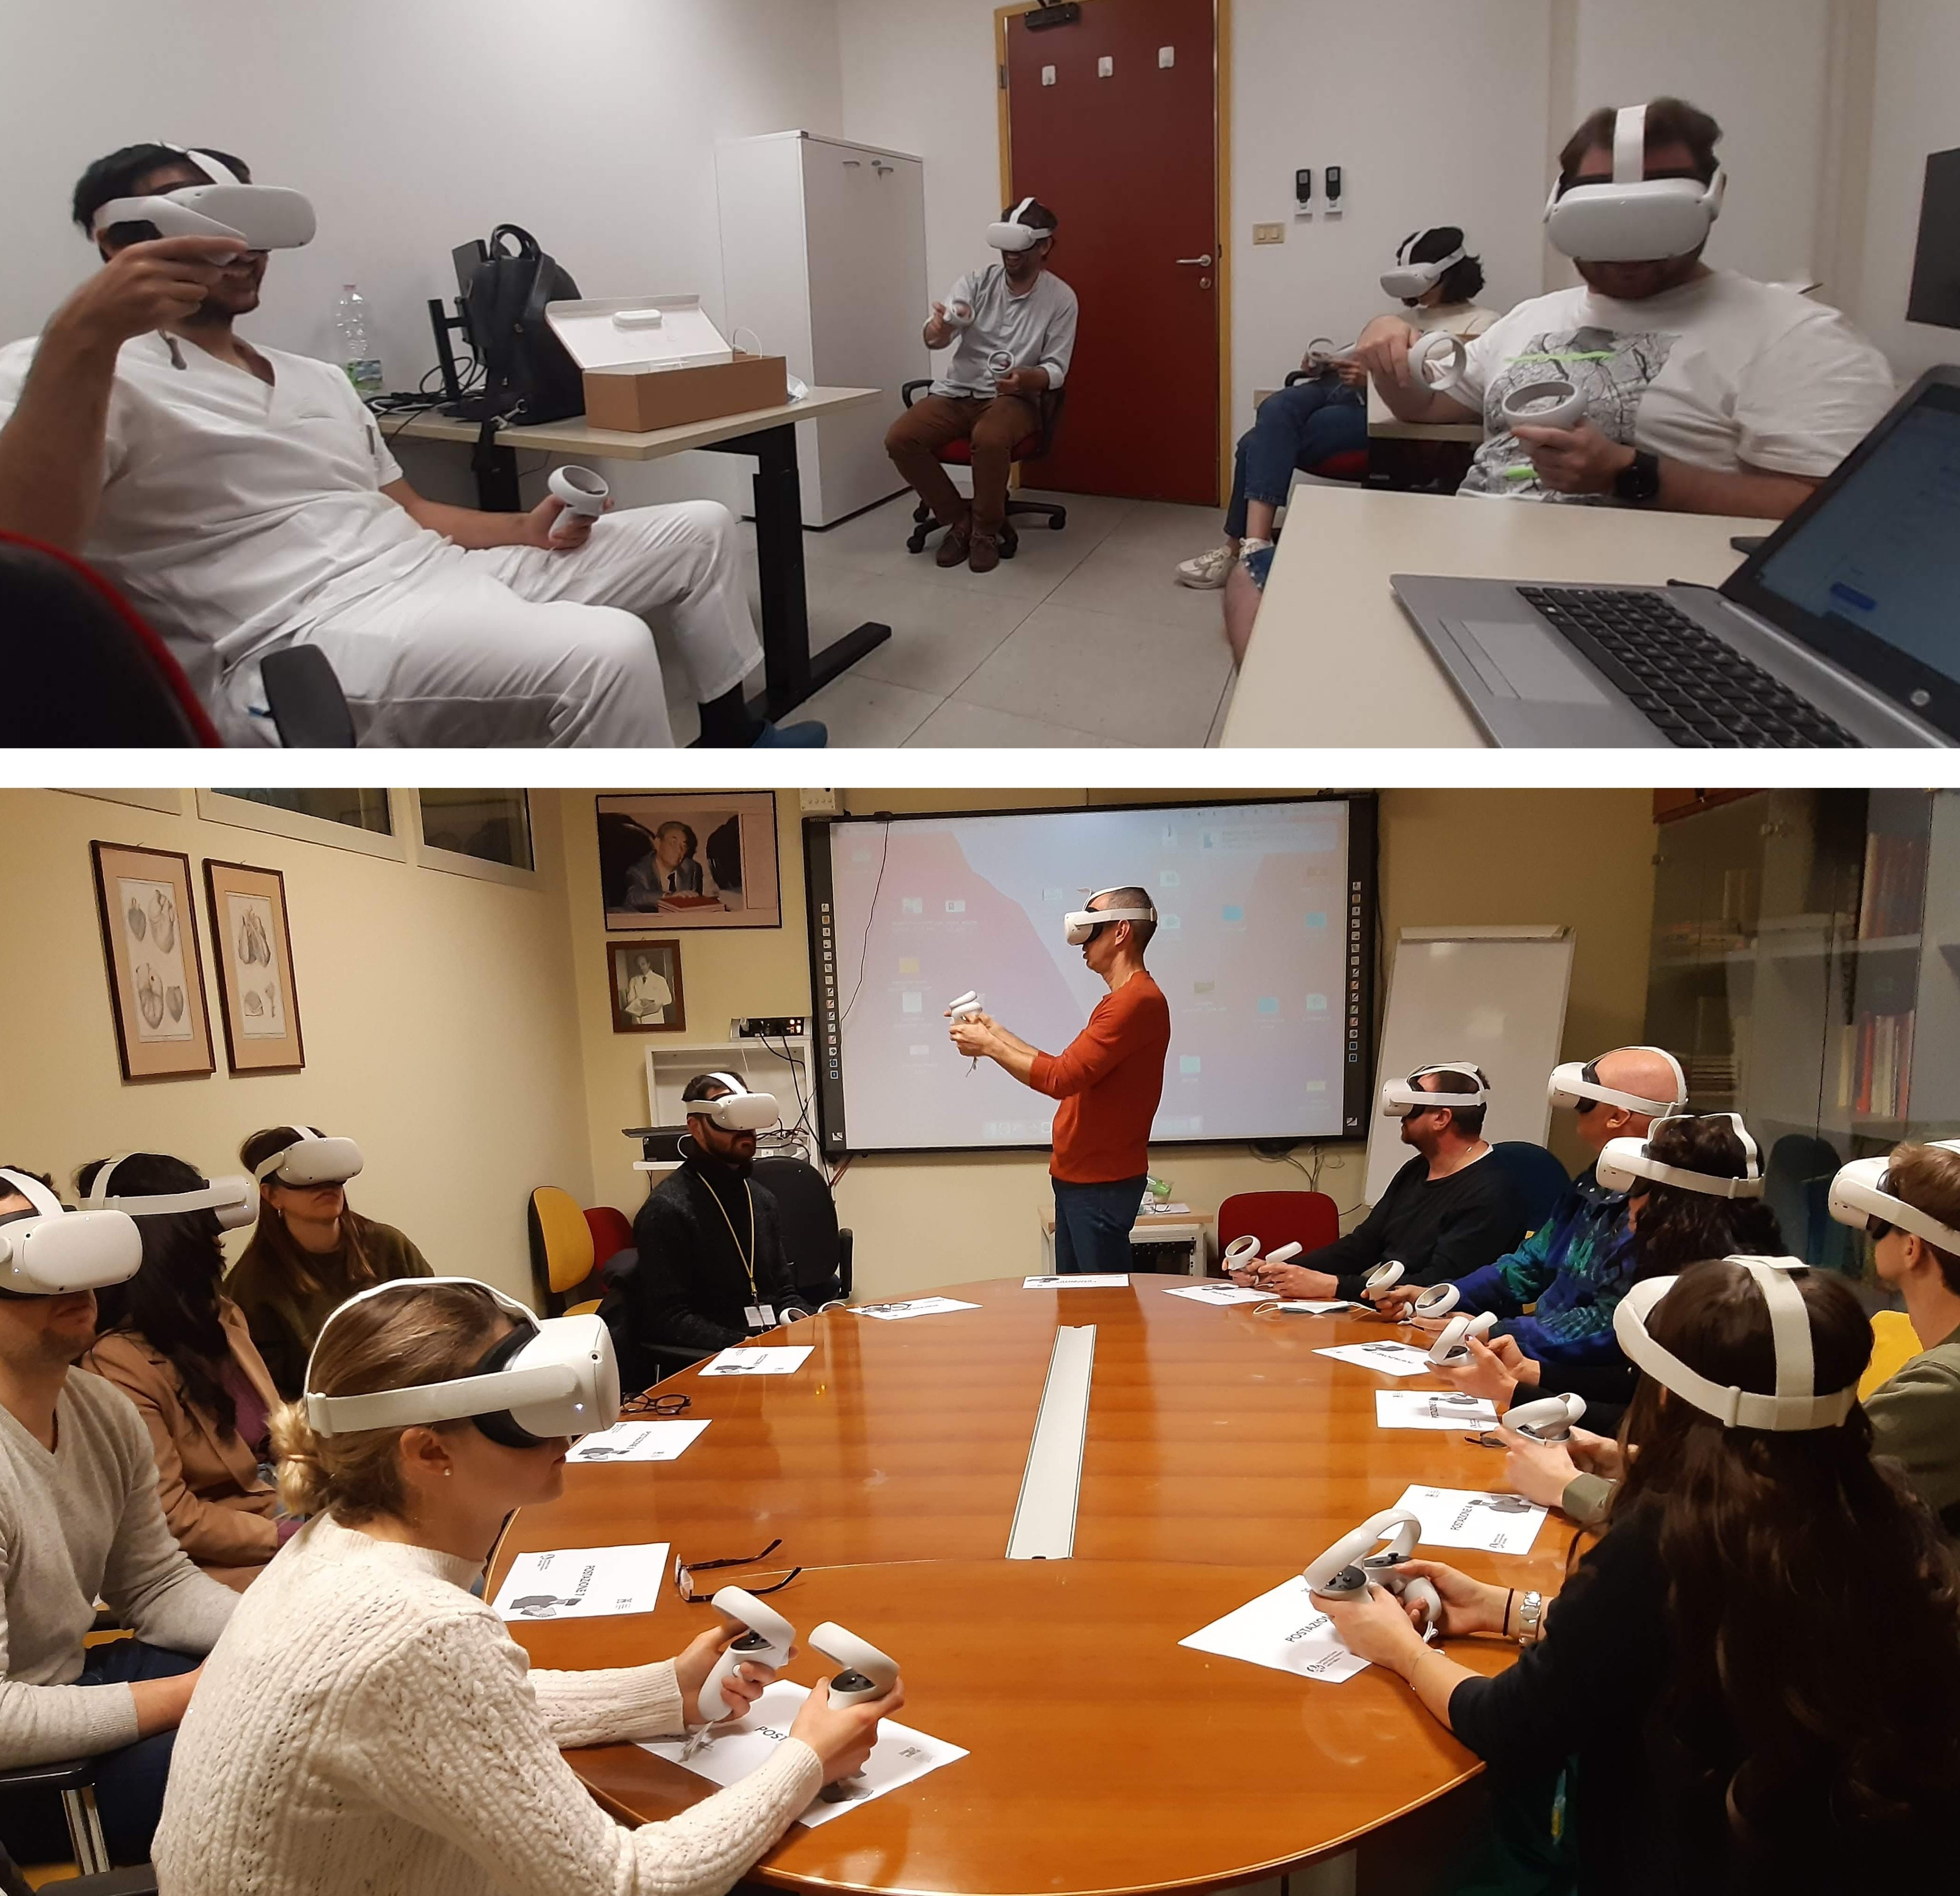
\includegraphics[width=0.96\textwidth]{testing.jpg}
  \caption{Testing session}
  \label{fig:testing}
\end{figure}

\section{Science4All}
\noindent
A special mention goes to the test of the application during the event Science4all hold in Padova in September 2024.
Science4All is a science outreach and inclusion software in Padua, aimed at making complex scientific topics accessible to a broad audience,
from young people to adults without a scientific background.\\
During the 2024 event, the \ac{VR} app was presented in the 3D printing section focused on medical applications.
For the occasion, considering the young age of the intended public, a specially designed environment Fig.[\ref{fig:science4all}].
The environment was designed to allow an operator to hide the hearts by shrinking them and concealing them within the office equipment in the room. A group of three children could then try to find all the hidden hearts.
By doing so, we allowed children to try the \ac{HMD}, for many, it was their first time experiencing \ac{VR}. They had the opportunity to view a heart model, exploring both the exterior and interior in detail.
Both children and parents were captivated by the app capabilities and the medical use case for which it was developed.\\
This provided valuable insights into additional use cases, new features, and bugs, thanks to the children's feedback and imagination, which will be useful for future development.


\begin{figure}[hb]
  \centering
  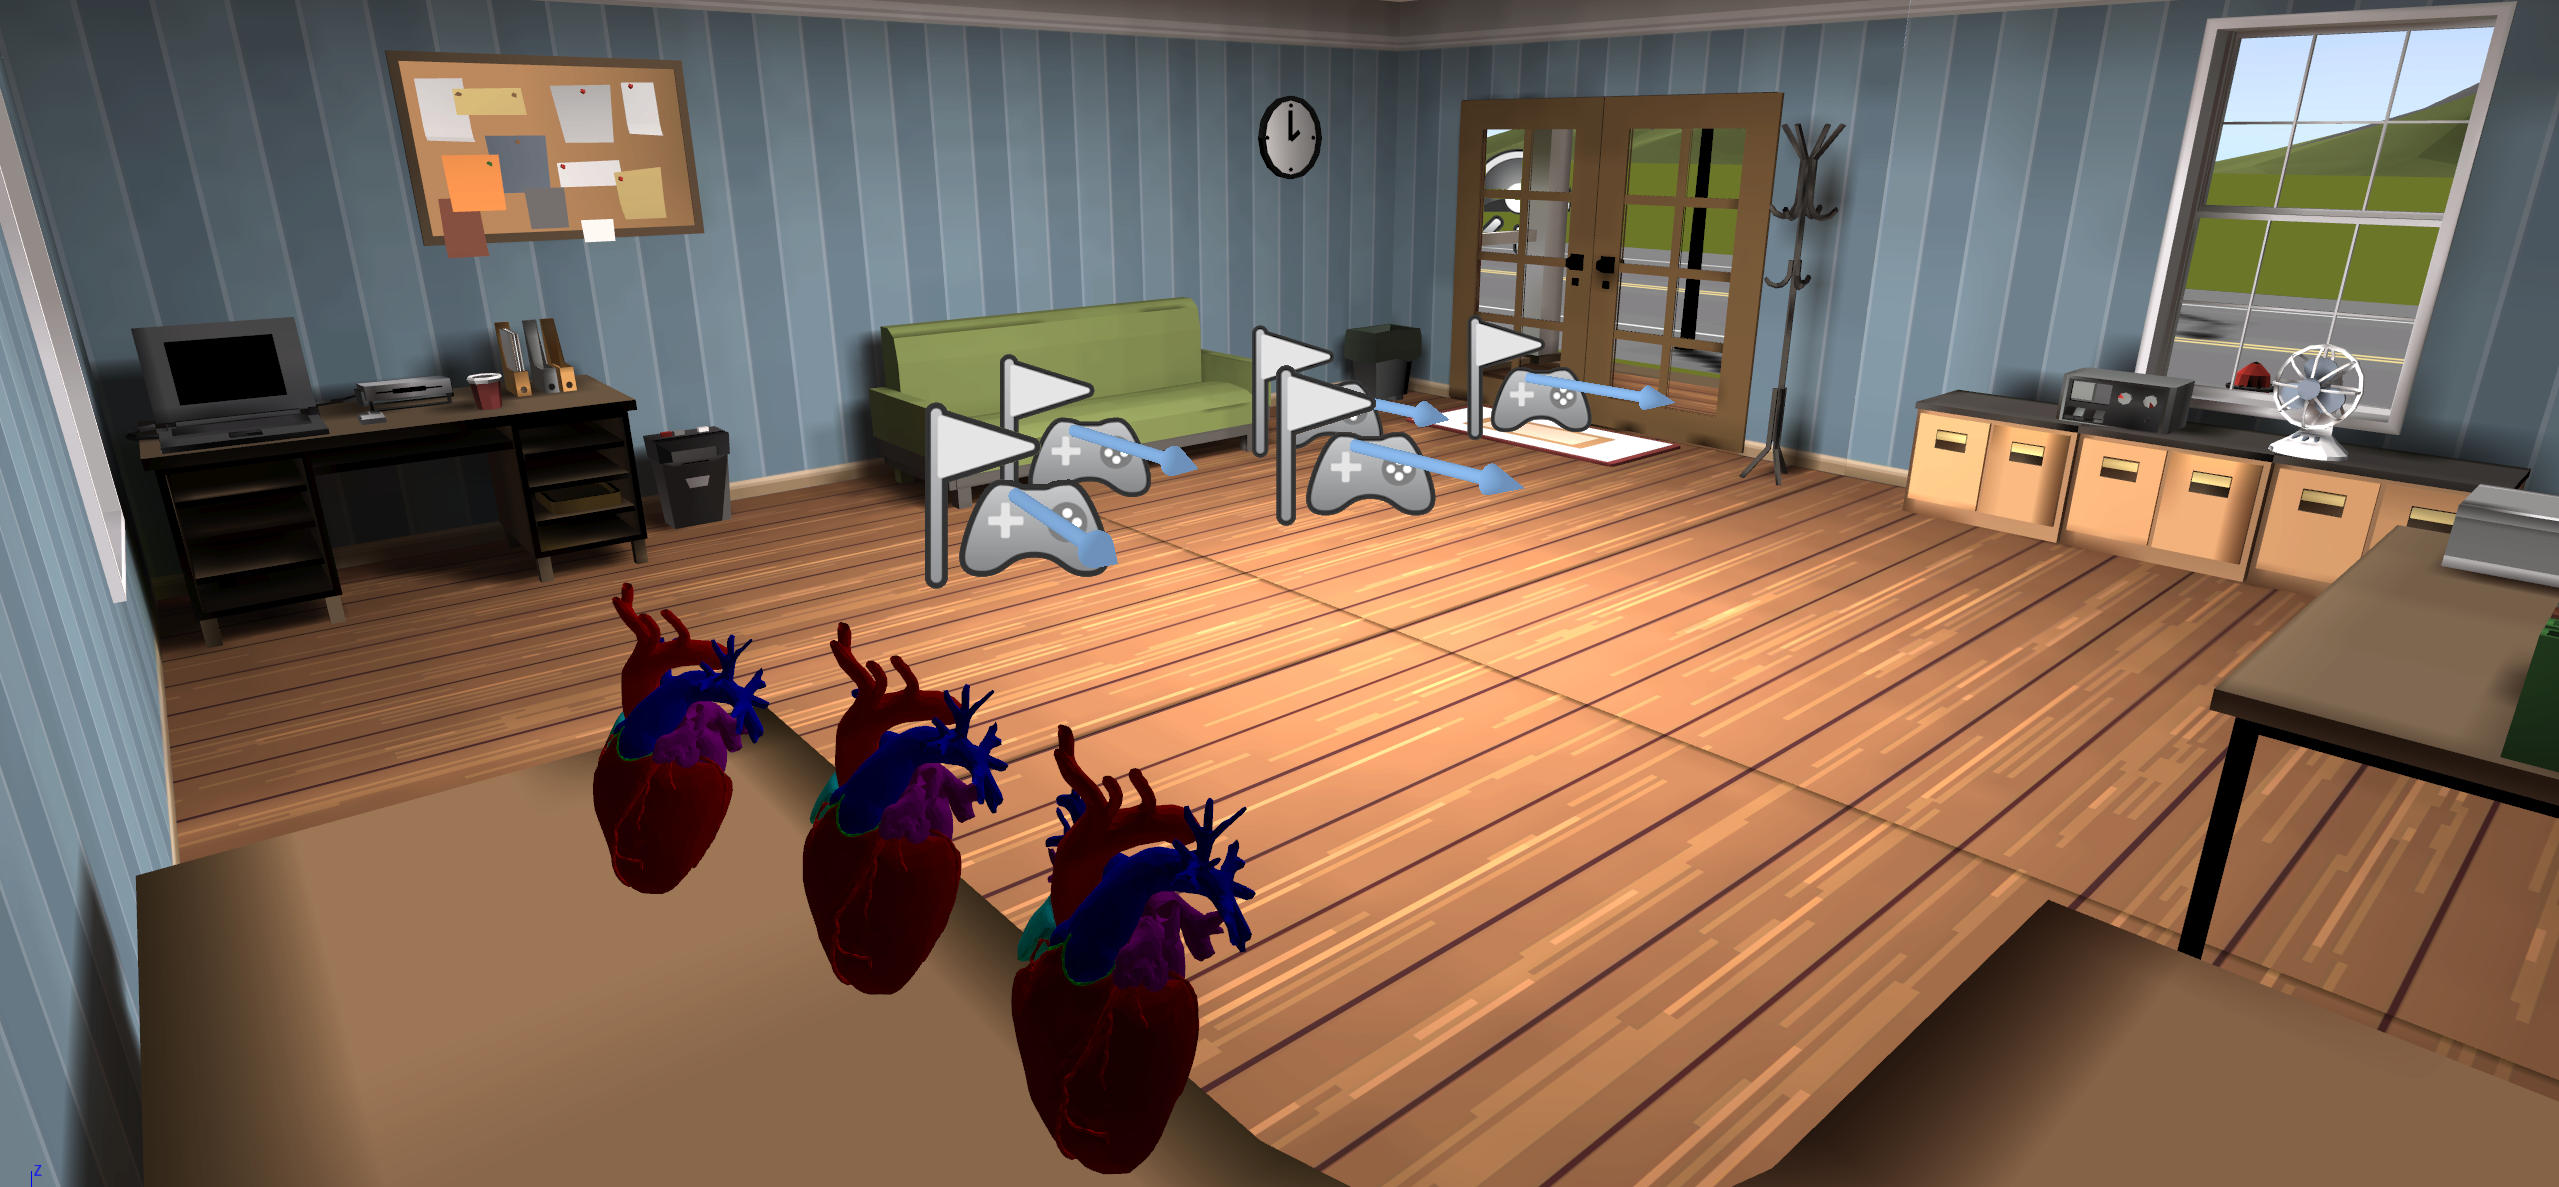
\includegraphics[width=0.96\textwidth]{vrScreenshot/science4all.png}
  \caption{Science4All environment}
  \label{fig:science4all}
\end{figure}